Besides the lexical model, we also use an acoustic model to predict the punctuation.
The acoustic model is based on prosodic features, such as pauses and pitch level.
In the following the training and evaluation of the acoustic model is shown in detail.

\subsection{Training instance generation}

Many researches are using pauses, pitch levels, and energy levels for prediction punctuation.
%Thus, we decided to also use this kind of features.
The pitch level encodes the volume of the speaker, whereas the energy level describes the amount of power the speaker is using in his voice.
To obtain those values from the \texttt{.sph} files in our data set, we first have to convert those files into \texttt{.wav} files.
For that, we used a sound processing program called \emph{SoX}.
Having the \texttt{.wav} files, we can extract the pitch and energy level from them using different libraries.
For generating the pitch level the library \emph{aubio}\footnote{\url{http://aubio.org/}} is used.
The output is a file containing two columns: The first columns is the time in seconds in the talk and the second column is the pitch level of that second.
The library \emph{Yaafe}\footnote{\url{yaafe.sourceforge.net/}} is used for extracting the energy levels from the \texttt{.wav} files.
The output from \emph{Yaafe} contains one column with energy values.
One line in the output file represents the energy level in \texttt{1 / sample rate} intervals.

Together with the \texttt{.ctm} files, we can now create the training instances.
The process of generating the training instances is shown in Figure~\ref{fig:overview_acoustic}.

\begin{figure}[ht]
    \centering
    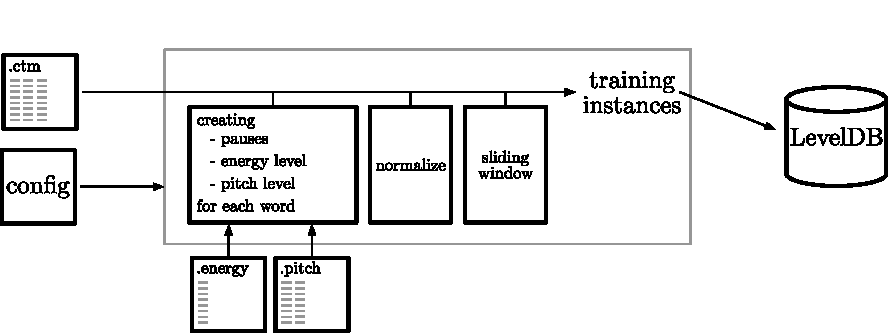
\includegraphics[width=0.8\textwidth]{img/overview_accoustic.pdf}
    \caption{Creating the training instance for the acoustic model. The pause feature is extracted from the \texttt{.ctm} files, the pitch level feature from the \texttt{.pitch} files and the energy level feature from the \texttt{.energy} file. All features are normalized to a mean 0 and a variance of 1. Like in the lexical model, a sliding window is used to create the final training instances.}
    \label{fig:overview_acoustic}
\end{figure}

The \texttt{.ctm} files hold the information of sentence boundaries.
Unfortunately, we do not have any information about other punctuation marks besides periods in those files.
Therefore, the acoustic model will be only able to predict periods.

Having the \texttt{.ctm} files the first step in the training instance generation is to extract the words with their corresponding start time and duration.
Additionally, the sentence boundaries are stored to obtain the gold standard.
% TODO: we tokenize again for having a better pos-tagging, replace i with I ???
When all words of a talk have been read, the pauses before and after each word are calculated.
Afterwards the \texttt{.energy} and \texttt{.pitch} files are parsed.
The energy and pitch level is mapped to the word, which was spoken at the time mentioned in the files.
It can happen, that multiple energy and pitch levels are mapped to one word.
In that case, the average value over all those energy/pitch levels belonging to one word is taken as final energy/pitch level for that word.

Furthermore, we filter the pitch values.
The voice frequency of a typical adult male ranges from 85 to 180 Hz, a typical adult female has a range from 165 to 255 Hz.
A lot of values in the pitch files lay far over those values, because of the background noise recorded in the talk.
Thus, we decided to filter all pitch levels, which are above 300 Hz.

In the end, we have the following four features for our acoustic model:
\begin{itemize}
	\item the duration of the pause before a word
	\item the duration of the pause after a word
	\item the average energy level of a word
	\item the average pitch level of a word.
\end{itemize}
In the next step the features are normalized to a mean of zero and a variance of one.

As in the lexical model, we use a sliding window to create the training instances.
The \texttt{config} file hold the information about the size of the window and the position of the punctuation.
Using the gold standard we obtained from the \texttt{.ctm} files, the training instance with the corresponding class (\textsc{None} or \textsc{Period}) are created.
The training instances are then written to a LevelDB in a last step.

\subsection{Neural Network}

%TODO: Hinge loss
We used the same model as for the lexical model, except in the input and the output layer.
For the input layer, we only have four features per word, compared to 314 features in the lexical layer.
So, for example, a window size of eight leads to 32 features.
In the last layer, we only use two dimensions instead of three, because we only have two classes: \textsc{None} and \textsc{Period}.

\begin{figure}[ht]
    \centering
    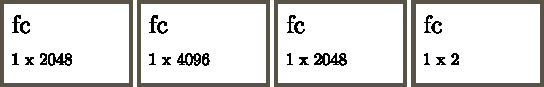
\includegraphics[width=0.6\textwidth]{img/net_acoustic.pdf}
    \caption{Network architecture consisting of four fully connected layers of the acoustic model.}
    \label{fig:net_acoustic}
\end{figure}


\subsection{Results and Evaluation}

As mentioned before, we can only evaluate the model on \textsc{Period}s, as we do not have ground truth data for the commas.
Again we evaluated different window sizes and punctuation positions.
Figure~\ref{audio_eval} shows the F-measure for all experiments.
Note that the y-axis has been capped to show differences better.
Interestingly, the combination of window size eight and punctuation position four is again the best combination.

\begin{figure}[ht]
    \centering
    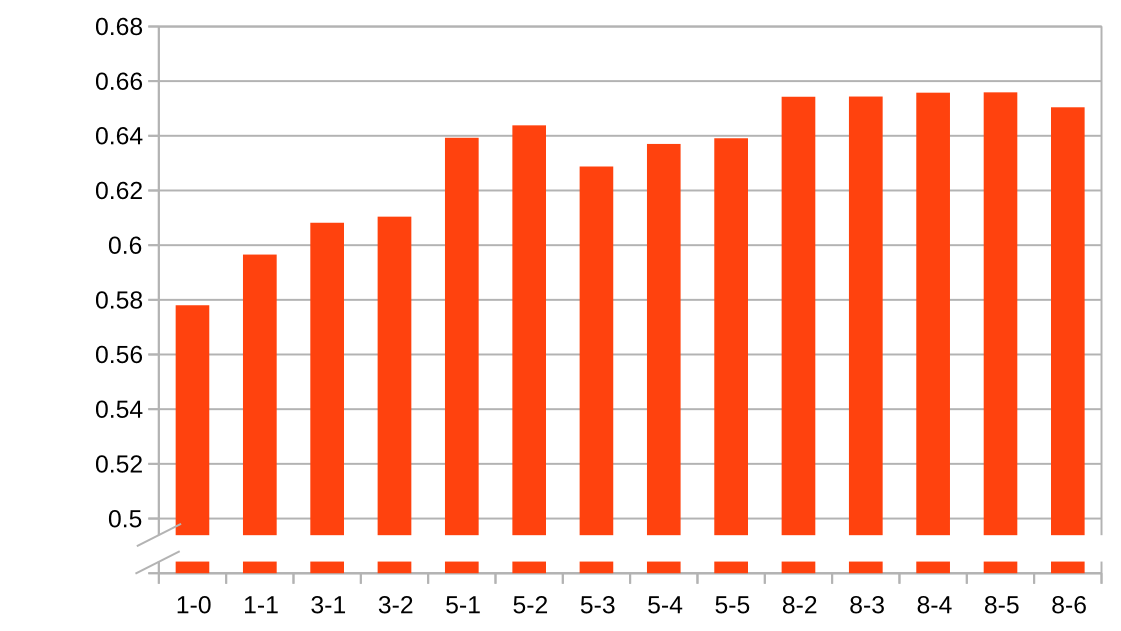
\includegraphics[width=0.5\textwidth]{img/audio_parameter_eval.png}
    \caption{}
    \label{audio_eval}
\end{figure}
